% ==============================================================================
% 第 25 章：非结构驱动的递归 (Chapter 25: Recursion without Structure)
% ==============================================================================

\chapter{非结构驱动的递归}
\label{sec:ch25_nonstandard}

至此，你已经设计了大量采用\term{结构型递归（structural recursion）}的函数。设计这类函数时，你清楚地知道必须审视主输入的数据定义。如果该输入由自引用数据定义来描述，那么函数在形式上就会自然而在数据定义引用自身之处调用自身。

本章将介绍两个采用不同递归方式的示例程序。它们生动地展示了需要某种“顿悟”（eureka）的问题——从直观朴素的想法到精妙深刻的洞见各不相同。

\section{脱离数据结构的递归}
\label{sec:25_1}

设想你加入了 DrRacket 开发团队。团队正在研发一项协作分享服务，旨在支持程序员之间的协同工作。具体而言，DrRacket 的下一个版本将允许 ISL 程序员在多台计算机之间共享其 DrRacket 定义区的内容。每当一位程序员修改代码缓冲区时，更新后的 DrRacket 就会将定义区的内容广播给参与该分享会话的所有 DrRacket 实例。

\begin{notebox}[样例问题]
你的任务是设计 \code{bundle} 函数，负责将定义区的内容打包以便广播。DrRacket 将内容作为 \code{1String}（单字符字符串）列表交付。该函数的任务是将离散的“字符”打包成若干数据块（chunk），进而生成一个由给定长度（称为块大小 \code{chunk size}）的字符串组成的列表。
\end{notebox}

如你所见，问题叙述几乎直接给出了签名，并不需要专门定义新的数据：

\begin{lstlisting}[language=BSL]
; [List-of 1String] N -> [List-of String]
; 将 s 中的字符按长度 n 切块打包为字符串列表
(define (bundle s n)
  '())
\end{lstlisting}

目的说明重新组织了问题描述中的语句，并使用了虚拟函数头中的形参名称。

第三步是编写功能示例。给定一个 \code{1String} 列表：

\begin{lstlisting}[language=BSL]
(list "a" "b" "c" "d" "e" "f" "g" "h")
\end{lstlisting}

如果我们要求 \code{bundle} 将这个列表按两两成对打包（即 $n$ 为 2），那么预期结果应为如下列表：

\begin{lstlisting}[language=BSL]
(list "ab" "cd" "ef" "gh")
\end{lstlisting}

现在，如果 $n$ 改为 3，就会多出一个剩余的“字符”。由于问题描述并未指明剩余字符应当如何处置，我们可以设想至少两种合理的情形：

\begin{itemize}
  \item 函数生成 \code{(list "abc" "def" "g")}；即它将最后一个字符视作多余的零头保留在末尾。
  \item 或者，它生成 \code{(list "a" "bcd" "efg")}，将开头的字符单独打包为一个字符串。
\end{itemize}

\begin{notebox}[思考停步]
你能想出至少一种其他合理的处理方案吗？
\end{notebox}

为了简单起见，我们选择第一种方案作为预期结果，并写下相应的单元测试：

\begin{lstlisting}[language=BSL]
(check-expect (bundle (explode "abcdefg") 3)
              (list "abc" "def" "g"))
\end{lstlisting}

注意这里使用了 \code{explode}，它使得测试用例更加清晰易读。

示例与测试还必须涵盖数据定义边界处的情形。在此语境下，边界显然意味着传递给 \code{bundle} 的列表长度不足一个完整的块大小：

\begin{lstlisting}[language=BSL]
(check-expect (bundle '("a" "b") 3) (list "ab"))
\end{lstlisting}

这也意味着我们必须考虑当传入 \code{'()} 时 \code{bundle} 的行为。为简便起见，我们选择 \code{'()} 作为预期输出：

\begin{lstlisting}[language=BSL]
(check-expect (bundle '() 3) '())
\end{lstlisting}

另一种自然的选择是要求返回 \code{'("")}。你能看出其他可能吗？

设计模板这一步揭示了一个事实：传统的结构化方法在这里行不通。图~\ref{fig:bundle-templates} 展示了四种可能的模板。由于 \code{bundle} 的两个参数都是复杂数据，前两个模板将其中一个参数视为原子数据。这显然不对，因为函数必须同时拆解这两个参数。第三个模板假定两个参数以步调一致（lockstep）的方式同步递归，这看似接近——但 \code{bundle} 显然需要定期将块大小重置为其初始值。最后一个模板假定两个参数独立递归，这意味着在每个阶段都有四种继续的方式。这最后一种设计将参数解耦得过于彻底，因为列表与计数必须协同处理。简而言之，面对这一设计问题，传统的结构化模板显得无能为力。

\begin{figure}[htbp]
  \centering
  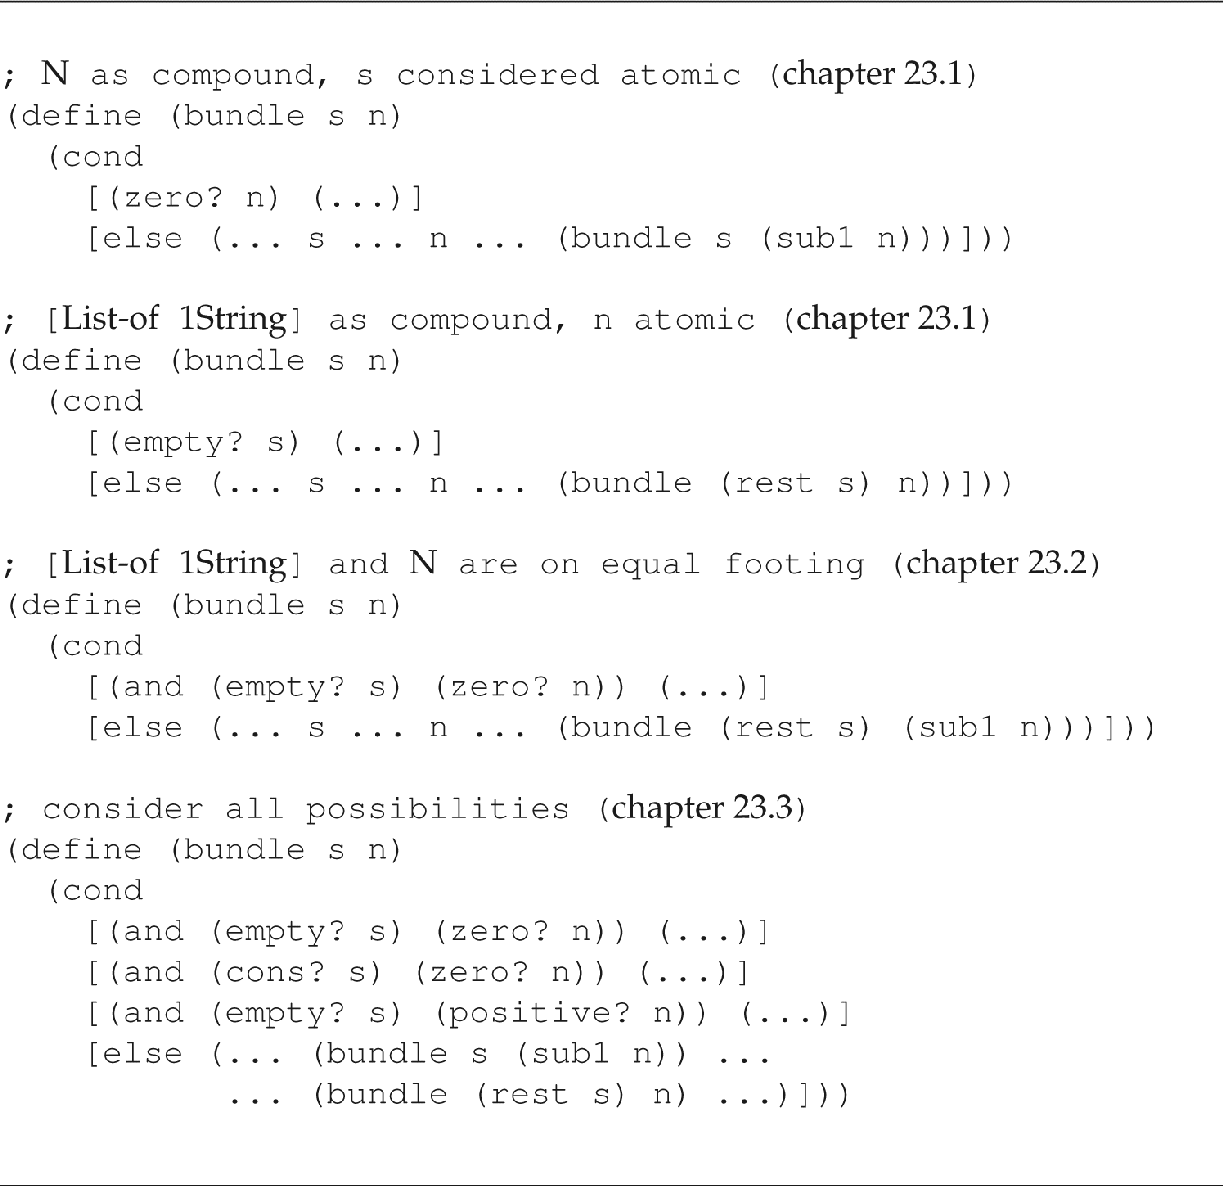
\includegraphics[width=0.85\textwidth]{images/00583.png}
  \caption{将字符串切块的四种无效模板}
  \label{fig:bundle-templates}
\end{figure}

图~\ref{fig:bundle-generative} 给出了 \code{bundle} 的完整定义。该定义使用了练习 395 中要求的 \code{drop} 和 \code{take} 函数；这些函数在标准库中也同样可用。为保持完整性，图中附带了它们的定义：\code{drop} 从列表头部至多丢弃 $n$ 个元素，而 \code{take} 则返回至多这么多个元素。借助这两个辅助函数，定义 \code{bundle} 就变得十分自然：

\begin{enumerate}
  \item 如果给定列表为 \code{'()}，结果如约返回 \code{'()}；
  \item 否则，\code{bundle} 使用 \code{take} 从 \code{s} 中取出前 $n$ 个 \code{1String}，并使用 \code{implode} 将其拼装成普通字符串；
  \item 接着，利用 \code{drop} 剔除前 $n$ 个元素，在缩短后的子列表上进行递归调用；
  \item 最后，使用 \code{cons} 将第 2 步得到的字符串与第 3 步得到的字符串列表组合起来，生成针对完整列表的最终结果。
\end{enumerate}

\begin{figure}[htbp]
  \centering
  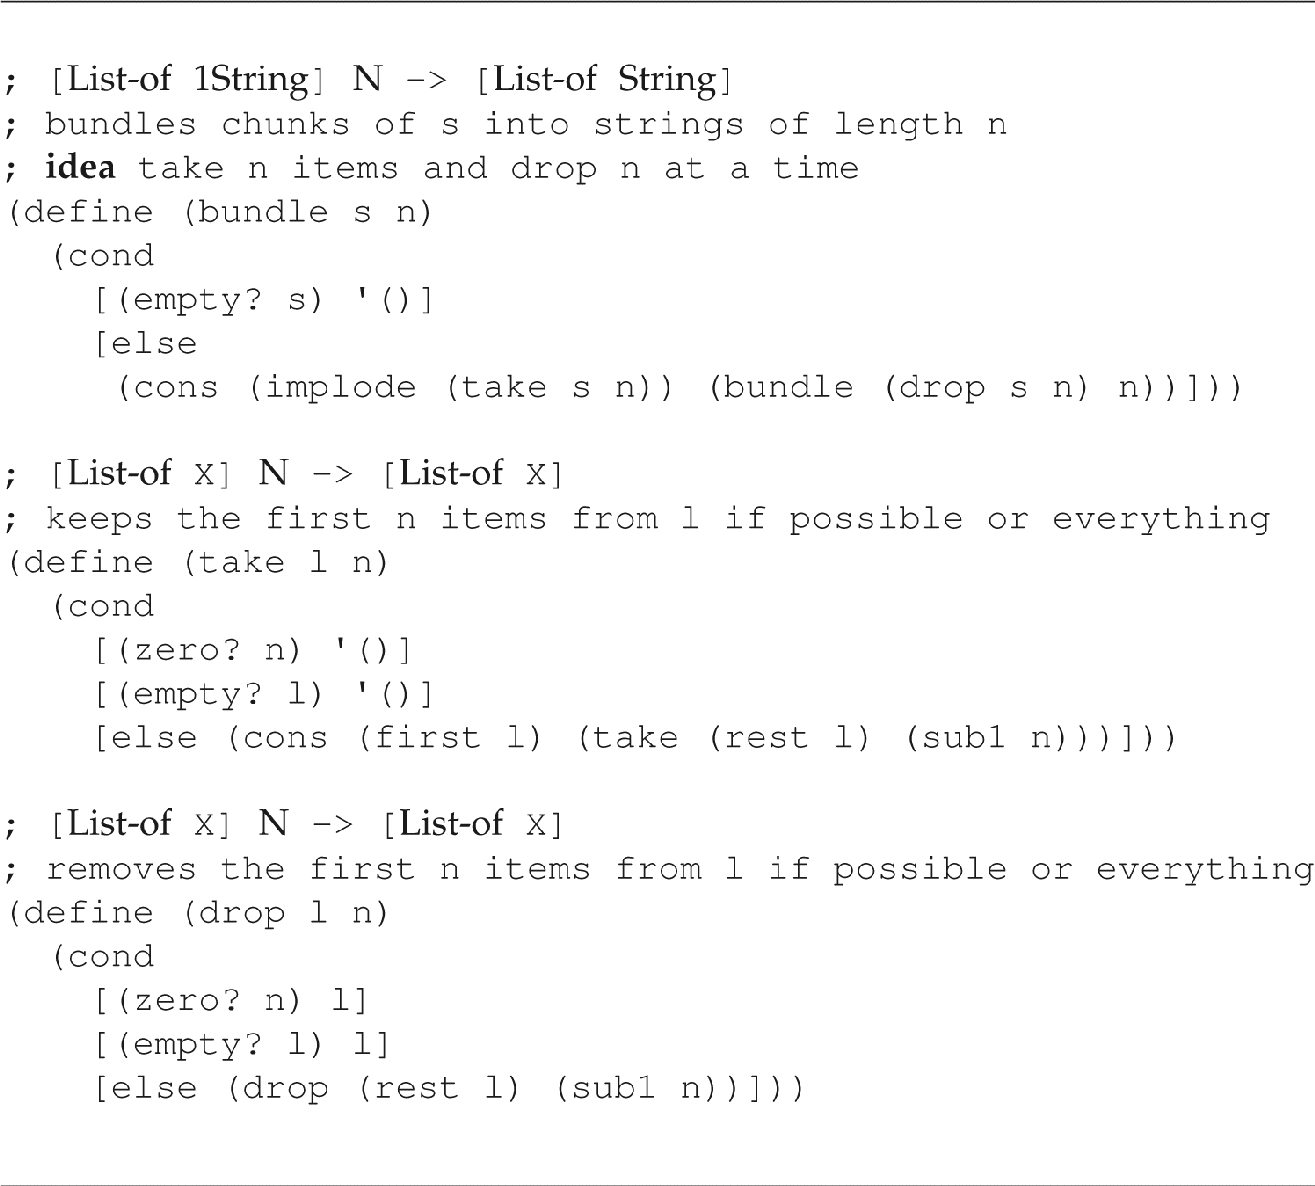
\includegraphics[width=0.85\textwidth]{images/00584.png}
  \caption{生成型递归：\code{bundle} 及其辅助函数的完整定义}
  \label{fig:bundle-generative}
\end{figure}

上述第 3 项凸显了 \code{bundle} 与本书前四部分中所有函数的根本差异。由于 \code{List-of} 的数据定义是通过在已有列表上 \code{cons} 一个元素来构造新列表的，因此前四部分中的所有函数都使用 \code{first} 和 \code{rest} 来解构非空列表。相比之下，\code{bundle} 使用了 \code{drop}，它一次性丢弃的不仅是一个元素，而是整整 $n$ 个元素。

尽管 \code{bundle} 的定义很不寻常，但其底层思想非常直观，与我们目前见过的函数也没有太大偏离。事实上，当块大小 $n$ 等于 1 时，\code{bundle} 就退化为标准的结构型递归定义。此外，\code{drop} 保证生成给定列表的一个组成部分，而不是某种任意打乱重排的版本。而这种思路正是下一节所要探讨的核心。

\begin{exercise}{调用 bundle 与边界情况}{421}\label{ex:421}
表达式 \code{(bundle '("a" "b" "c") 0)} 是对 \code{bundle} 函数的合法调用吗？它会产生什么结果？为什么？
\end{exercise}

\begin{exercise}{基于列表切块定义 bundle}{422}\label{ex:422}
定义函数 \code{list->chunks}。该函数接收任意数据的列表 \code{l} 以及自然数 \code{n}。函数的结果是大小为 \code{n} 的列表块的列表。每个块代表 \code{l} 中项的一个连续子序列。

请使用 \code{list->chunks} 通过函数组合来定义 \code{bundle}。
\end{exercise}

\begin{exercise}{基于字符串切片的 partition 函数}{423}\label{ex:423}
定义函数 \code{partition}。它接收一个字符串 \code{s} 和自然数 \code{n}。函数生成一个由长度为 \code{n} 的字符串切块组成的列表。

对于非空字符串 \code{s} 与正自然数 \code{n}，以下等式应当成立：
\begin{lstlisting}[language=BSL]
(equal? (partition s n) (bundle (explode s) n))
\end{lstlisting}
但请不要直接将该等式作为 \code{partition} 的定义，而应使用 \code{substring}。

\textbf{提示}：让 \code{partition} 对空字符串产生其自然的结果。对于 $n = 0$ 的情况，请参考练习~\ref{ex:421}。

\textbf{注}：相比 \code{bundle}，\code{partition} 函数更贴近协同 DrRacket 环境的实际需求。
\end{exercise}

\section{忽略结构的递归}
\label{sec:25_2}

回顾第 11 章中的 \code{sort>} 函数，它接收一个数字列表并按某种顺序（通常是升序或降序）重新排列。它的工作机制是将第一个数字插入到剩余列表排序后所得列表的合适位置。换言之，它是一个结构型递归函数，对自然递归的结果进行后处理。

霍尔（C. A. R. Hoare）的\term{快速排序算法（quick-sort algorithm）}则以一种截然不同的方式对列表进行排序，并成为了\term{生成型递归（generative recursion）}的经典范例。其底层的生成步骤采用了久经考验的\term{分治策略（divide-and-conquer strategy）}：将问题的非平凡实例划分为两个规模更小且相关的子问题；求解这两个子问题；然后将子问题的解合并为原问题的解。就快速排序算法而言，其中间目标是将数字列表划分为两个子列表：
\begin{itemize}
  \item 一个包含所有严格小于第一个数字的元素；
  \item 另一个包含所有严格大于第一个数字的元素。
\end{itemize}
随后，使用快速排序算法对这两个较小的子列表进行递归排序。一旦两个子列表完成排序，就将它们组合起来，并将第一个元素放置在中间。鉴于其特殊的枢纽角色，列表中的第一个元素被称为\term{基准元（pivot item，或枢轴元）}。

为了深入理解快速排序的工作原理，我们通过一个具体例子来演练对 \code{(list 11 8 14 7)} 进行快速排序的过程。图~\ref{fig:quicksort-diagram} 以图形化方式直观展示了这一过程。整张图由上半部分的“划分阶段”（divide phase）与下半部分的“合并解决阶段”（conquer phase）组成。

\begin{figure}[htbp]
  \centering
  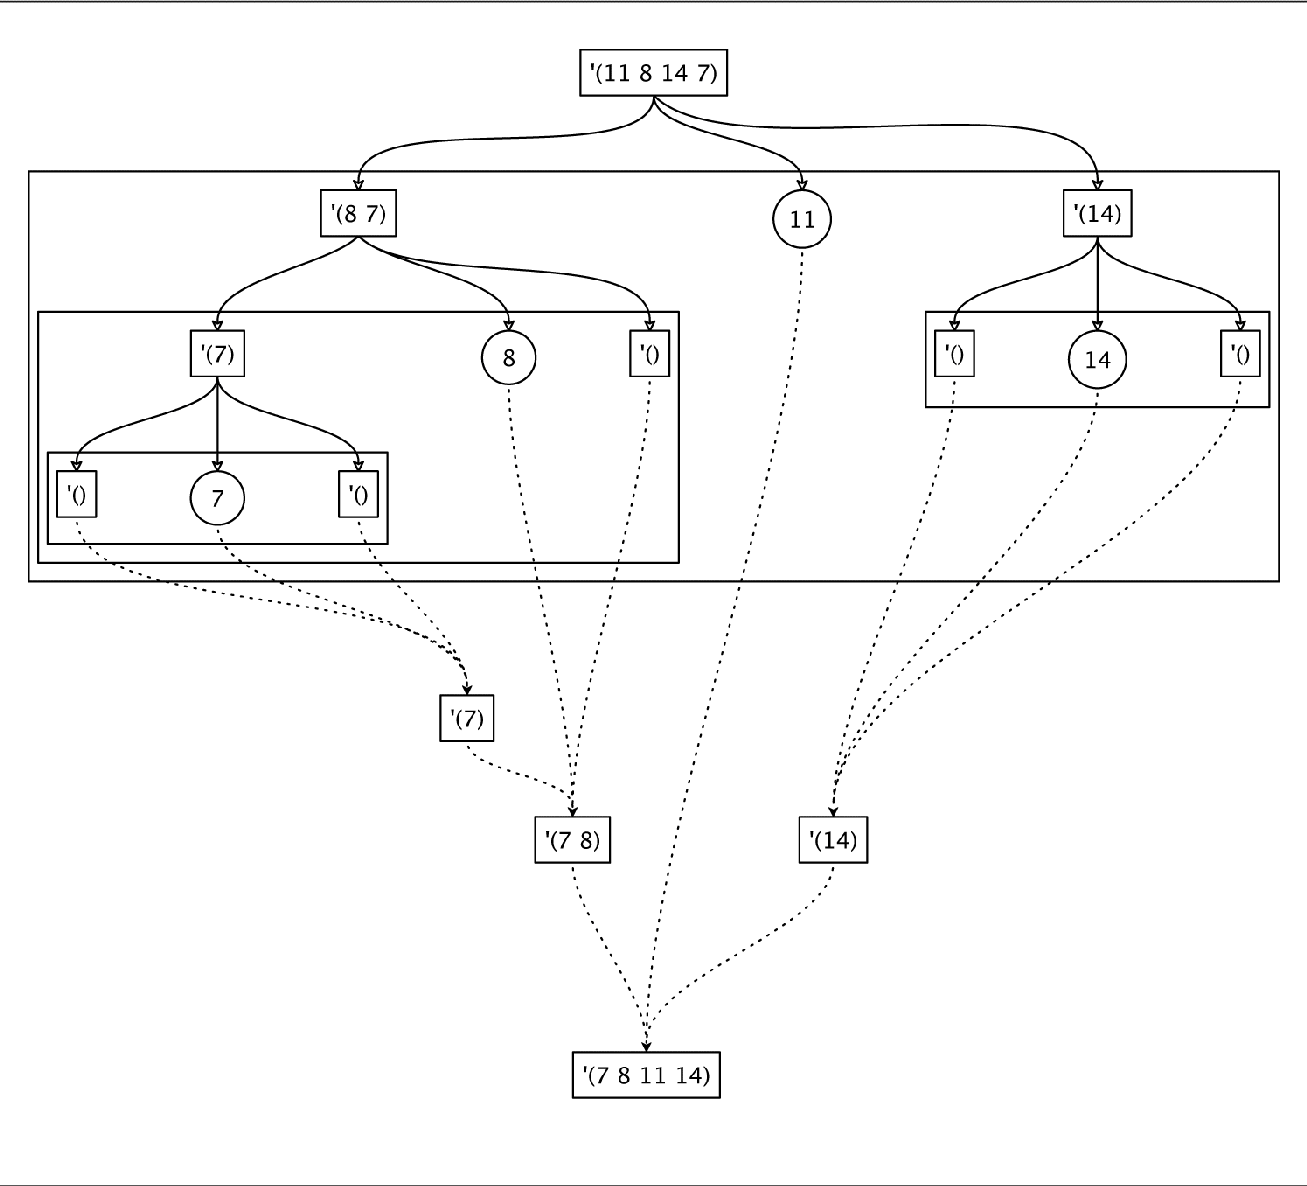
\includegraphics[width=0.85\textwidth]{images/00585.png}
  \caption{快速排序算法的图解过程}
  \label{fig:quicksort-diagram}
\end{figure}

划分阶段由带框列表与实线箭头表示。每个带框列表引出三条箭头，指向一个包含三部分的框：中间是带圆圈的基准元，其左侧是比基准元小的数字列表，其右侧是比基准元大的数字列表。每一步都至少隔离出一个数字作为基准元，这意味着左右两个相邻列表的长度都严格小于给定的原列表。因此，整个划分过程必然会终止。

考虑输入为 \code{(list 11 8 14 7)} 的第一步：基准元是 \code{11}。将列表划分为小于和大于 \code{11} 的元素，分别得到 \code{(list 8 7)} 和 \code{(list 14)}。划分阶段的其余步骤以类似方式工作。当所有数字都被隔离为基准元时，划分阶段结束。此时，只要从左向右读取所有的基准元，就能直接读出最终的排序结果。

合并解决阶段由虚线箭头与带框列表表示。三条箭头汇入每个结果框：中间一条来自基准元，左侧来自较小数字排序后的结果，右侧来自较大数字排序后的结果。每一步都将至少一个数字（即基准元）加入结果列表，这意味着列表朝向图的底部不断增长。底部的框就是顶部给定列表的有序排列。

观察最左上角的合并步骤：它将基准元 \code{7} 与两个空列表合并，得到 \code{'(7)}。再下一级对应于隔离出 \code{8} 的划分步骤，从而生成 \code{'(7 8)}。合并解决阶段的每一层级都镜像映射了划分阶段的对应层级。归根结底，整个过程是递归的。

\begin{exercise}{绘制快速排序追踪图}{424}\label{ex:424}
针对列表 \code{(list 11 9 2 18 12 14 4 1)}，绘制一张类似于图~\ref{fig:quicksort-diagram} 的快速排序执行图。
\end{exercise}

既然我们已经充分理解了快速排序的思想，就可以将其翻译为 ISL+ 代码。显而易见，\code{quick-sort<} 区分两种情况：如果输入是 \code{'()}，由于空列表本身已经有序，直接产生 \code{'()}；否则，执行生成型递归。这种情形划分提示了如下 \code{cond} 表达式：

\begin{lstlisting}[language=BSL]
; [List-of Number] -> [List-of Number]
; 生成 alon 的升序排列版本
; 假设所有数字互不相同
(define (quick-sort< alon)
  (cond
    [(empty? alon) '()]
    [else (... (first alon) ... (rest alon) ...)]))
\end{lstlisting}

第一种情况的结果不言自明。对于第二种情况，当 \code{quick-sort<} 的输入为非空列表时，算法利用首个元素将列表的其余部分划分为两个子列表：一个包含所有小于基准元的项，另一个包含所有大于基准元的项。

由于剩余列表的长度未知，我们将列表划分的任务委托给两个辅助函数：\code{smallers} 和 \code{largers}。它们遍历列表，分别过滤出小于和大于基准元的元素。因此，每个辅助函数都接收两个参数：一个数字列表和一个数字。设计这两个函数是一次标准结构型递归的练习。你可以尝试独立编写，或者阅读图~\ref{fig:quicksort-full} 中给出的定义。

\begin{figure}[htbp]
  \centering
  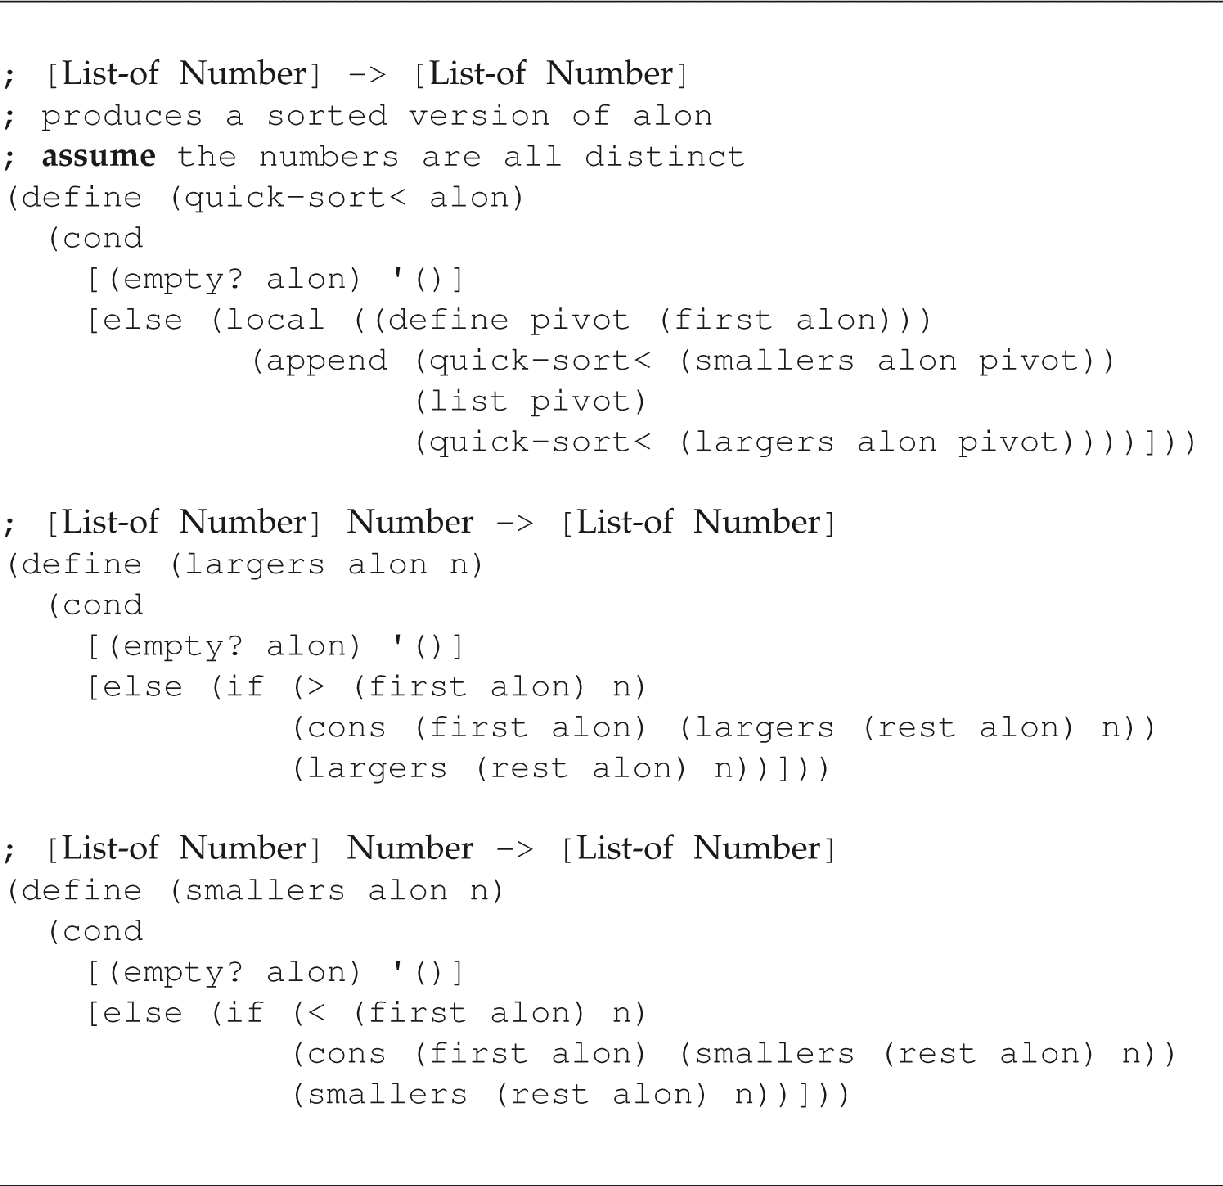
\includegraphics[width=0.85\textwidth]{images/00587.png}
  \caption{快速排序算法及辅助函数}
  \label{fig:quicksort-full}
\end{figure}

这两个子列表分别使用 \code{quick-sort<} 进行独立排序，这构成了递归调用，具体表现为如下两个表达式：
\begin{enumerate}
  \item \code{(quick-sort< (smallers alon pivot))}：对所有小于基准元的元素进行排序；
  \item \code{(quick-sort< (largers alon pivot))}：对所有大于基准元的元素进行排序。
\end{enumerate}

一旦 \code{quick-sort<} 获得了两个子列表排序后的版本，就必须按恰当的顺序将两部分与基准元拼接起来：首先是所有小于 \code{pivot} 的项，接着是 \code{pivot}，最后是所有大于它的项。由于第一部分和最后一部分已经排好序，\code{quick-sort<} 只需简单使用 \code{append}：

\begin{lstlisting}[language=BSL]
(append (quick-sort< (smallers (rest alon) pivot))
        (list pivot)
        (quick-sort< (largers (rest alon) pivot)))
\end{lstlisting}

图~\ref{fig:quicksort-full} 包含了完整的程序；在继续阅读之前请仔细研读它。

有了具体的函数定义后，我们可以手工推导前面示例的求值过程：

\begin{lstlisting}[language=BSL]
  (quick-sort< (list 11 8 14 7))
== (append (quick-sort< (list 8 7))
           (list 11)
           (quick-sort< (list 14)))
== (append (append (quick-sort< (list 7))
                   (list 8)
                   (quick-sort< '()))
           (list 11)
           (quick-sort< (list 14)))
== (append (append (append (quick-sort< '())
                           (list 7)
                           (quick-sort< '()))
                   (list 8)
                   '())
           (list 11)
           (quick-sort< (list 14)))
== ...
\end{lstlisting}

这一推演展示了排序过程的核心步骤，即划分步骤、递归排序步骤以及三部分的拼接。从该推演中，很容易看出 \code{quick-sort<} 是如何实现图~\ref{fig:quicksort-diagram} 中所示过程的。

图~\ref{fig:quicksort-diagram} 与手动计算都清晰表明：\code{quick-sort<} 完全忽略了给定列表的既有结构。第一次递归作用于原始列表中相隔甚远的两个数字，而第二次递归作用于列表的第三个元素。这些递归调用绝非随机产生，但它们显然不再依赖于数据定义的自然结构。

将 \code{quick-sort<} 的组织结构与第 11 章中的 \code{sort>} 函数进行对比：后者的设计严格遵循结构化设计配方，生成逐个处理列表项的程序。而通过对列表进行划分，\code{quick-sort<} 能够极大地加快列表排序的过程——其代价则是不再使用简单的 \code{first} 与 \code{rest} 遍历。

\begin{exercise}{为 smallers 与 largers 编写目的说明}{425}\label{ex:425}
为图~\ref{fig:quicksort-full} 中的 \code{smallers} 与 \code{largers} 辅助函数清晰阐述其目的说明。
\end{exercise}

\begin{exercise}{单元素列表的平凡情形优化}{426}\label{ex:426}
完成上述手工推导过程。仔细检查求值步骤会揭示 \code{quick-sort<} 的一个额外的平凡情形（trivial case）：每当 \code{quick-sort<} 接收只有一个元素的列表时，它都可以直接原样返回该列表。毕竟，只有一个元素的列表本身必然是有序的。

请修改 \code{quick-sort<} 以利用这一观察结果。重新推导上述示例。修改后的算法节省了多少个求值步骤？
\end{exercise}

\begin{exercise}{结合插入排序的阈值混合排序}{427}\label{ex:427}
虽然在多数情况下 \code{quick-sort<} 能迅速缩小问题规模，但对于极小规模的问题，它的开销却相对过大。因此，工程实践中常使用 \code{quick-sort<} 来减小问题规模，当列表缩减到足够小时则切换到另一种排序函数。

请开发一个 \code{quick-sort<} 的改进版本：当输入列表的长度低于某个阈值时，切换使用 \code{sort<}（即第 11.3 节中 \code{sort>} 的升序适配版本）。
\end{exercise}

\begin{exercise}{处理包含重复数字的列表}{428}\label{ex:428}
如果传给 \code{quick-sort<} 的输入列表中包含多个相同的数字，算法返回的列表长度将严格小于输入的长度。为什么会出现这种现象？请修正该问题，使得输出列表与输入列表长度相同且保留所有重复项。
\end{exercise}

\begin{exercise}{使用 filter 定义 smallers 与 largers}{429}\label{ex:429}
使用抽象函数 \code{filter} 重新定义 \code{smallers} 与 \code{largers}。
\end{exercise}

\begin{exercise}{单一比较算子与抽象快速排序}{430}\label{ex:430}
开发 \code{quick-sort<} 的一个变体，它只使用单一比较函数（例如 \code{<}）。其划分步骤将给定的列表 \code{alon} 划分为一个包含所有小于基准元的元素列表，以及另一个包含所有不小于基准元的元素列表。

使用 \code{local} 将程序封装为一个单一函数。随后对该函数进行抽象，使其接收一个列表和一个通用比较谓词作为参数。
\end{exercise}
